\begin{figure}[H]
    \centering
    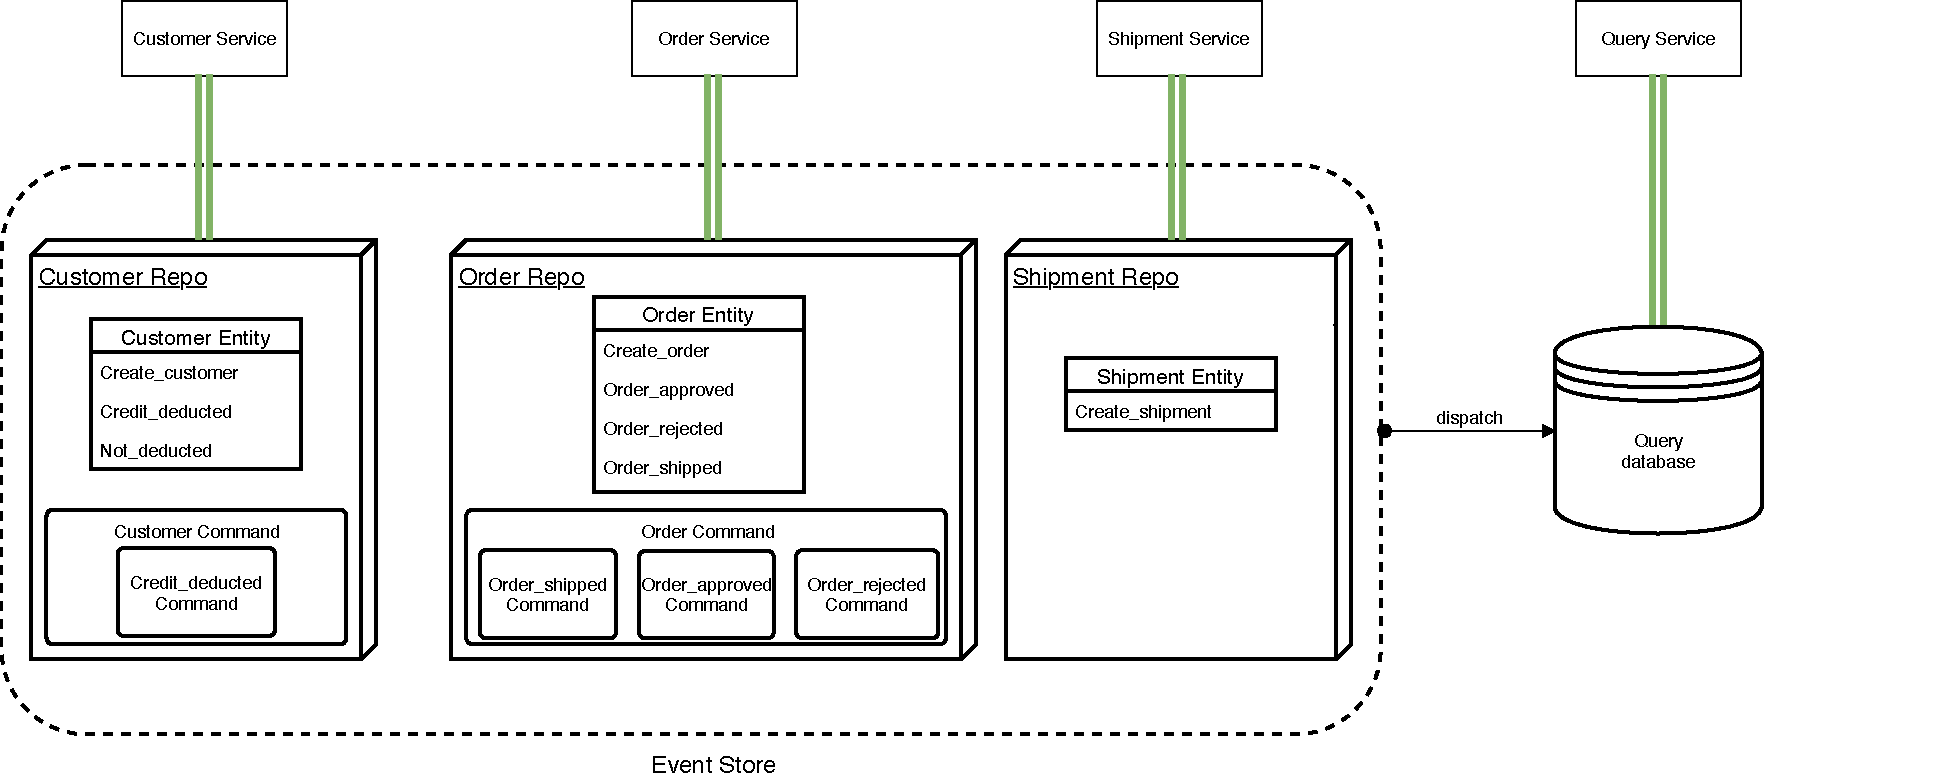
\includegraphics[width=17cm]{assets/arch.pdf}
    \nocaptionrule \caption{\label{fig:arch} Overall structure of the e-commerce prototype}
\end{figure}

To evaluate the usability of Axon and Eventuate frameworks, we take on both quantitative and qualitative approaches. We implemented a dummy e-commerce system with a business logic that requires multi-database transaction in a rational manner and is very common in the real world. The general workflow of the system is the following:

% {\fontfamily{pcr}\selectfont
\begin{enumerate}
    \item Create a customer with name and credit limit
    \item Create order
    \begin{itemize}
        \item If order amount does not exceed customer credit limit, approve order and subtract credit.
        \item If order amount exceeds customer credit limit, reject order and maintain credit unchanged
    \end{itemize}
    \item If order is approved, create shipment, order status change as shipped.
\end{enumerate}
% }

The system starts off with no data consistency guarantees. As the experiment, we implement data consistency using the two frameworks separately by two team members (Nana and Xin). To evaluate the usability quantitatively, we plan to record the following data:

\begin{itemize}
    \item Total lines of Java source code (SLOC)
    \item Size of the systems on the disk
    \item Estimated time taken to implement the improvement
    \item Total time spent on the web (also separately on GitHub, StackOverflow, documentation website and other related reference sites)
    \item Documentation: total number of words, estimated coverage of the framework APIs
    \item Performance and stability: we use Artillery to load test the two implementations using Axon and Eventuate. If significant difference detected, we can also report system resource usages (CPU usage and network respond time).
\end{itemize}

Qualitatively, we will report our experience using the two frameworks, provide some more anecdotal cases of tasks such as reading the documentation, and showcase some snippets of code to discuss their API designs.
